
%% bare_conf.tex
%% V1.3
%% 2007/01/11
%% by Michael Shell
%% See:
%% http://www.michaelshell.org/
%% for current contact information.
%%
%% This is a skeleton file demonstrating the use of IEEEtran.cls
%% (requires IEEEtran.cls version 1.7 or later) with an IEEE conference paper.
%%
%% Support sites:
%% http://www.michaelshell.org/tex/ieeetran/
%% http://www.ctan.org/tex-archive/macros/latex/contrib/IEEEtran/
%% and
%% http://www.i eee.org/

%%*************************************************************************
%% Legal Notice:
%% This code is offered as-is without any warranty either expressed or
%% implied; without even the implied warranty of MERCHANTABILITY or
%% FITNESS FOR A PARTICULAR PURPOSE! 
%% User assumes all risk.
%% In no event shall IEEE or any contributor to this code be liable for
%% any damages or losses, including, but not limited to, incidental,
%% consequential, or any other damages, resulting from the use or misuse
%% of any information contained here.
%%
%% All comments are the opinions of their respective authors and are not
%% necessarily endorsed by the IEEE.
%%
%% This work is distributed under the LaTeX Project Public License (LPPL)
%% ( http://www.latex-project.org/ ) version 1.3, and may be freely used,
%% distributed and modified. A copy of the LPPL, version 1.3, is included
%% in the base LaTeX documentation of all distributions of LaTeX released
%% 2003/12/01 or later.
%% Retain all contribution notices and credits.
%% ** Modified files should be clearly indicated as such, including  **
%% ** renaming them and changing author support contact information. **
%%
%% File list of work: IEEEtran.cls, IEEEtran_HOWTO.pdf, bare_adv.tex,
%%                    bare_conf.tex, bare_jrnl.tex, bare_jrnl_compsoc.tex
%%*************************************************************************

% *** Authors should verify (and, if needed, correct) their LaTeX system  ***
% *** with the testflow diagnostic prior to trusting their LaTeX platform ***
% *** with production work. IEEE's font choices can trigger bugs that do  ***
% *** not appear when using other class files.                            ***
% The testflow support page is at:
% http://www.michaelshell.org/tex/testflow/



% Note that the a4paper option is mainly intended so that authors in
% countries using A4 can easily print to A4 and see how their papers will
% look in print - the typesetting of the document will not typically be
% affected with changes in paper size (but the bottom and side margins will).
% Use the testflow package mentioned above to verify correct handling of
% both paper sizes by the user's LaTeX system.
%
% Also note that the "draftcls" or "draftclsnofoot", not "draft", option
% should be used if it is desired that the figures are to be displayed in
% draft mode.
%
\documentclass[conference]{IEEEtran}
\IEEEoverridecommandlockouts
\usepackage{makeidx}
\usepackage{amsmath}
\usepackage{graphicx}
\usepackage{algorithm2e}

\newtheorem{principle}{Principle}
\newtheorem{definition}{Definition}
\newtheorem{theorem}{Theorem}
\def\network{{\sf N}}

\newcommand{\tuple}[2] {\langle #1,#2\rangle}
% Add the compsoc option for Computer Society conferences.
%
% If IEEEtran.cls has not been installed into the LaTeX system files,
% manually specify the path to it like:
% \documentclass[conference]{../sty/IEEEtran}





% Some very useful LaTeX packages include:
% (uncomment the ones you want to load)


% *** MISC UTILITY PACKAGES ***
%
%\usepackage{ifpdf}
% Heiko Oberdiek's ifpdf.sty is very useful if you need conditional
% compilation based on whether the output is pdf or dvi.
% usage:
% \ifpdf
%   % pdf code
% \else
%   % dvi code
% \fi
% The latest version of ifpdf.sty can be obtained from:
% http://www.ctan.org/tex-archive/macros/latex/contrib/oberdiek/
% Also, note that IEEEtran.cls V1.7 and later provides a builtin
% \ifCLASSINFOpdf conditional that works the same way.
% When switching from latex to pdflatex and vice-versa, the compiler may
% have to be run twice to clear warning/error messages.






% *** CITATION PACKAGES ***
%
%\usepackage{cite}
% cite.sty was written by Donald Arseneau
% V1.6 and later of IEEEtran pre-defines the format of the cite.sty package
% \cite{} output to follow that of IEEE. Loading the cite package will
% result in citation numbers being automatically sorted and properly
% "compressed/ranged". e.g., [1], [9], [2], [7], [5], [6] without using
% cite.sty will become [1], [2], [5]--[7], [9] using cite.sty. cite.sty's
% \cite will automatically add leading space, if needed. Use cite.sty's
% noadjust option (cite.sty V3.8 and later) if you want to turn this off.
% cite.sty is already installed on most LaTeX systems. Be sure and use
% version 4.0 (2003-05-27) and later if using hyperref.sty. cite.sty does
% not currently provide for hyperlinked citations.
% The latest version can be obtained at:
% http://www.ctan.org/tex-archive/macros/latex/contrib/cite/
% The documentation is contained in the cite.sty file itself.






% *** GRAPHICS RELATED PACKAGES ***
%
\ifCLASSINFOpdf
  % \usepackage[pdftex]{graphicx}
  % declare the path(s) where your graphic files are
  % \graphicspath{{../pdf/}{../jpeg/}}
  % and their extensions so you won't have to specify these with
  % every instance of \includegraphics
  % \DeclareGraphicsExtensions{.pdf,.jpeg,.png}
\else
  % or other class option (dvipsone, dvipdf, if not using dvips). graphicx
  % will default to the driver specified in the system graphics.cfg if no
  % driver is specified.
  % \usepackage[dvips]{graphicx}
  % declare the path(s) where your graphic files are
  % \graphicspath{{../eps/}}
  % and their extensions so you won't have to specify these with
  % every instance of \includegraphics
  % \DeclareGraphicsExtensions{.eps}
\fi
% graphicx was written by David Carlisle and Sebastian Rahtz. It is
% required if you want graphics, photos, etc. graphicx.sty is already
% installed on most LaTeX systems. The latest version and documentation can
% be obtained at: 
% http://www.ctan.org/tex-archive/macros/latex/required/graphics/
% Another good source of documentation is "Using Imported Graphics in
% LaTeX2e" by Keith Reckdahl which can be found as epslatex.ps or
% epslatex.pdf at: http://www.ctan.org/tex-archive/info/
%
% latex, and pdflatex in dvi mode, support graphics in encapsulated
% postscript (.eps) format. pdflatex in pdf mode supports graphics
% in .pdf, .jpeg, .png and .mps (metapost) formats. Users should ensure
% that all non-photo figures use a vector format (.eps, .pdf, .mps) and
% not a bitmapped formats (.jpeg, .png). IEEE frowns on bitmapped formats
% which can result in "jaggedy"/blurry rendering of lines and letters as
% well as large increases in file sizes.
%
% You can find documentation about the pdfTeX application at:
% http://www.tug.org/applications/pdftex





% *** MATH PACKAGES ***
%
%\usepackage[cmex10]{amsmath}
% A popular package from the American Mathematical Society that provides
% many useful and powerful commands for dealing with mathematics. If using
% it, be sure to load this package with the cmex10 option to ensure that
% only type 1 fonts will utilized at all point sizes. Without this option,
% it is possible that some math symbols, particularly those within
% footnotes, will be rendered in bitmap form which will result in a
% document that can not be IEEE Xplore compliant!
%
% Also, note that the amsmath package sets \interdisplaylinepenalty to 10000
% thus preventing page breaks from occurring within multiline equations. Use:
%\interdisplaylinepenalty=2500
% after loading amsmath to restore such page breaks as IEEEtran.cls normally
% does. amsmath.sty is already installed on most LaTeX systems. The latest
% version and documentation can be obtained at:
% http://www.ctan.org/tex-archive/macros/latex/required/amslatex/math/





% *** SPECIALIZED LIST PACKAGES ***
%
%\usepackage{algorithmic}
% algorithmic.sty was written by Peter Williams and Rogerio Brito.
% This package provides an algorithmic environment fo describing algorithms.
% You can use the algorithmic environment in-text or within a figure
% environment to provide for a floating algorithm. Do NOT use the algorithm
% floating environment provided by algorithm.sty (by the same authors) or
% algorithm2e.sty (by Christophe Fiorio) as IEEE does not use dedicated
% algorithm float types and packages that provide these will not provide
% correct IEEE style captions. The latest version and documentation of
% algorithmic.sty can be obtained at:
% http://www.ctan.org/tex-archive/macros/latex/contrib/algorithms/
% There is also a support site at:
% http://algorithms.berlios.de/index.html
% Also of interest may be the (relatively newer and more customizable)
% algorithmicx.sty package by Szasz Janos:
% http://www.ctan.org/tex-archive/macros/latex/contrib/algorithmicx/




% *** ALIGNMENT PACKAGES ***
%
%\usepackage{array}
% Frank Mittelbach's and David Carlisle's array.sty patches and improves
% the standard LaTeX2e array and tabular environments to provide better
% appearance and additional user controls. As the default LaTeX2e table
% generation code is lacking to the point of almost being broken with
% respect to the quality of the end results, all users are strongly
% advised to use an enhanced (at the very least that provided by array.sty)
% set of table tools. array.sty is already installed on most systems. The
% latest version and documentation can be obtained at:
% http://www.ctan.org/tex-archive/macros/latex/required/tools/


%\usepackage{mdwmath}
%\usepackage{mdwtab}
% Also highly recommended is Mark Wooding's extremely powerful MDW tools,
% especially mdwmath.sty and mdwtab.sty which are used to format equations
% and tables, respectively. The MDWtools set is already installed on most
% LaTeX systems. The lastest version and documentation is available at:
% http://www.ctan.org/tex-archive/macros/latex/contrib/mdwtools/


% IEEEtran contains the IEEEeqnarray family of commands that can be used to
% generate multiline equations as well as matrices, tables, etc., of high
% quality.


%\usepackage{eqparbox}
% Also of notable interest is Scott Pakin's eqparbox package for creating
% (automatically sized) equal width boxes - aka "natural width parboxes".
% Available at:
% http://www.ctan.org/tex-archive/macros/latex/contrib/eqparbox/





% *** SUBFIGURE PACKAGES ***
%\usepackage[tight,footnotesize]{subfigure}
% subfigure.sty was written by Steven Douglas Cochran. This package makes it
% easy to put subfigures in your figures. e.g., "Figure 1a and 1b". For IEEE
% work, it is a good idea to load it with the tight package option to reduce
% the amount of white space around the subfigures. subfigure.sty is already
% installed on most LaTeX systems. The latest version and documentation can
% be obtained at:
% http://www.ctan.org/tex-archive/obsolete/macros/latex/contrib/subfigure/
% subfigure.sty has been superceeded by subfig.sty.



%\usepackage[caption=false]{caption}
%\usepackage[font=footnotesize]{subfig}
% subfig.sty, also written by Steven Douglas Cochran, is the modern
% replacement for subfigure.sty. However, subfig.sty requires and
% automatically loads Axel Sommerfeldt's caption.sty which will override
% IEEEtran.cls handling of captions and this will result in nonIEEE style
% figure/table captions. To prevent this problem, be sure and preload
% caption.sty with its "caption=false" package option. This is will preserve
% IEEEtran.cls handing of captions. Version 1.3 (2005/06/28) and later 
% (recommended due to many improvements over 1.2) of subfig.sty supports
% the caption=false option directly:
%\usepackage[caption=false,font=footnotesize]{subfig}
%
% The latest version and documentation can be obtained at:
% http://www.ctan.org/tex-archive/macros/latex/contrib/subfig/
% The latest version and documentation of caption.sty can be obtained at:
% http://www.ctan.org/tex-archive/macros/latex/contrib/caption/




% *** FLOAT PACKAGES ***
%
%\usepackage{fixltx2e}
% fixltx2e, the successor to the earlier fix2col.sty, was written by
% Frank Mittelbach and David Carlisle. This package corrects a few problems
% in the LaTeX2e kernel, the most notable of which is that in current
% LaTeX2e releases, the ordering of single and double column floats is not
% guaranteed to be preserved. Thus, an unpatched LaTeX2e can allow a
% single column figure to be placed prior to an earlier double column
% figure. The latest version and documentation can be found at:
% http://www.ctan.org/tex-archive/macros/latex/base/



%\usepackage{stfloats}
% stfloats.sty was written by Sigitas Tolusis. This package gives LaTeX2e
% the ability to do double column floats at the bottom of the page as well
% as the top. (e.g., "\begin{figure*}[!b]" is not normally possible in
% LaTeX2e). It also provides a command:
%\fnbelowfloat
% to enable the placement of footnotes below bottom floats (the standard
% LaTeX2e kernel puts them above bottom floats). This is an invasive package
% which rewrites many portions of the LaTeX2e float routines. It may not work
% with other packages that modify the LaTeX2e float routines. The latest
% version and documentation can be obtained at:
% http://www.ctan.org/tex-archive/macros/latex/contrib/sttools/
% Documentation is contained in the stfloats.sty comments as well as in the
% presfull.pdf file. Do not use the stfloats baselinefloat ability as IEEE
% does not allow \baselineskip to stretch. Authors submitting work to the
% IEEE should note that IEEE rarely uses double column equations and
% that authors should try to avoid such use. Do not be tempted to use the
% cuted.sty or midfloat.sty packages (also by Sigitas Tolusis) as IEEE does
% not format its papers in such ways.





% *** PDF, URL AND HYPERLINK PACKAGES ***
%
%\usepackage{url}
% url.sty was written by Donald Arseneau. It provides better support for
% handling and breaking URLs. url.sty is already installed on most LaTeX
% systems. The latest version can be obtained at:
% http://www.ctan.org/tex-archive/macros/latex/contrib/misc/
% Read the url.sty source comments for usage information. Basically,
% \url{my_url_here}.





% *** Do not adjust lengths that control margins, column widths, etc. ***
% *** Do not use packages that alter fonts (such as pslatex).         ***
% There should be no need to do such things with IEEEtran.cls V1.6 and later.
% (Unless specifically asked to do so by the journal or conference you plan
% to submit to, of course. )


% correct bad hyphenation here
\hyphenation{}


\begin{document}
%
% paper title
% can use linebreaks \\ within to get better formatting as desired
\title{Extended Structural Balance Theory for Modeling Trust in Social
  Networks}


% author names and affiliations
% use a multiple column layout for up to three different
% affiliations
\author{\IEEEauthorblockN{Yi Qian}
\IEEEauthorblockA{Department of Computer Science\\
Rensselaer Polytechnic Institute\\
%110 8th Street, Troy, NY 12180\\
Email: qiany3@rpi.edu}
\and
\IEEEauthorblockN{Sibel Adal{\i}}
\IEEEauthorblockA{Department of Computer Science\\
Rensselaer Polytechnic Institute\\
%110 8th Street, Troy, NY 12180\\
Email: adalis@rpi.edu} \thanks{ This research is supported through the
  authors' participation in the Network Science Collaborative
  Technology Alliance (NS-CTA) sponsored by the U.S.~Army Research
  Laboratory under Agreement Number W911NF-09-2-0053.  The content of
  this paper does not necessarily reflect the position or policy of
  the U.S.~Government, no official endorsement should be inferred or
  implied.
%% Research was sponsored by the Army Research Laboratory and was
%% accomplished under Cooperative Agreement Number W911NF-09-2-0053. The
%% views and conclusions contained in this document are those of the
%% authors and should not be interpreted as representing the official
%% policies, either expressed or implied, of the Army Research Laboratory
%% or the U.S. Government. The U.S. Government is authorized to reproduce
%% and distribute reprints for Government purposes notwithstanding any
%% copyright notation here on.
We also would like to thank T. DuBois for sharing the implementation
details of his algorithm.
}}

% conference papers do not typically use \thanks and this command
% is locked out in conference mode. If really needed, such as for
% the acknowledgment of grants, issue a \IEEEoverridecommandlockouts
% after \documentclass

% for over three affiliations, or if they all won't fit within the width
% of the page, use this alternative format:
% 
%\author{\IEEEauthorblockN{Michael Shell\IEEEauthorrefmark{1},
%Homer Simpson\IEEEauthorrefmark{2},
%James Kirk\IEEEauthorrefmark{3}, 
%Montgomery Scott\IEEEauthorrefmark{3} and
%Eldon Tyrell\IEEEauthorrefmark{4}}
%\IEEEauthorblockA{\IEEEauthorrefmark{1}School of Electrical and Computer Engineering\\
%Georgia Institute of Technology,
%Atlanta, Georgia 30332--0250\\ Email: see http://www.michaelshell.org/contact.html}
%\IEEEauthorblockA{\IEEEauthorrefmark{2}Twentieth Century Fox, Springfield, USA\\
%Email: homer@thesimpsons.com}
%\IEEEauthorblockA{\IEEEauthorrefmark{3}Starfleet Academy, San Francisco, California 96678-2391\\
%Telephone: (800) 555--1212, Fax: (888) 555--1212}
%\IEEEauthorblockA{\IEEEauthorrefmark{4}Tyrell Inc., 123 Replicant Street, Los Angeles, California 90210--4321}}




% use for special paper notices
%\IEEEspecialpapernotice{(Invited Paper)}




% make the title area
\maketitle


\begin{abstract}
%\boldmath
Modeling trust in very large social networks is a hard problem due to
the highly noisy nature of these networks that span trust
relationships from many different contexts, based on judgments of
reliability, dependability and competence and the relationships vary
in their level of strength. In this paper, we introduce a new extended
balance theory as a foundational theory of trust in networks. Our
theory preserves the distinctions between trust and distrust as
suggested in the literature, but also incorporates the notion of
relationship strength which can be expressed as either discrete
categorical values, as pairwise comparisons or as metric
distances. Our model is novel, has sound social and psychological
basis, and captures the classical balance theory as a special case. We
then propose a convergence model, describing how an imbalanced network
evolves towards new balance and formulate the convergence problem of a
social network as a Metric Multidimensional Scaling (MDS) optimization
problem.  Finally, we show how the convergence model can be used to
predict edge signs in social networks, and justify our theory through
experiments on real datasets.
\end{abstract}
% IEEEtran.cls defaults to using nonbold math in the Abstract.
% This preserves the distinction between vectors and scalars. However,
% if the conference you are submitting to favors bold math in the abstract,
% then you can use LaTeX's standard command \boldmath at the very start
% of the abstract to achieve this. Many IEEE journals/conferences frown on
% math in the abstract anyway.

% no keywords




% For peer review papers, you can put extra information on the cover
% page as needed:
% \ifCLASSOPTIONpeerreview
% \begin{center} \bfseries EDICS Category: 3-BBND \end{center}
% \fi
%
% For peerreview papers, this IEEEtran command inserts a page break and
% creates the second title. It will be ignored for other modes.
\IEEEpeerreviewmaketitle


\section{Introduction}
Modeling trust in very large social networks is a hard problem due to
the highly noisy nature of these networks. These networks span trust
relationships from many different contexts, based on judgments of
reliability, dependability and
competence~\cite{Adali:2013}. Furthermore, trust relationships vary in
their level of strength as participants may or may not know each other
well. One specific problem of interest is inferring new relationships
and making recommendations based on existing relationships. To this
date, many algorithms for such prediction problems are based on
machine learning methods. These methods generate multiple structural
features from the known relationships, and then use these features to
classify the unknown
relationships~\cite{golbeck:distrust2011}\cite{Guha:04}\cite{Leskovec:2010}. In
particular, the concept of structural balance is widely applied when
developing these algorithms. For example, Leskovec et al. generate a
class of ``triad features'' in their prediction algorithm, i.e. a pair
of relationships constraining a third
relationship~\cite{Leskovec:2010}. They also use the structural
balance as a touchstone to see the congruence between their practical
results and the long studied theory. In essence, the transitivity of
trust and distrust within a triad can be easily inferred from the
balance theory. Other algorithms~\cite{golbeck:distrust2011} make use
of similar assumptions without explicit mention of balance theory in
which trust and distrust relationships are mapped to metric distances
on a continuous range. While these algorithms show strong prediction
performance, there is no underlying theory that explains how
structural balance can be mapped to metric distances. That is, a
theory that stands as the cornerstone of trust prediction is
missing. Without such a theory, it is not possible to develop
principled algorithms and study to which degree a specific network
conforms to the theory, and to illustrate the importance of various
balance related properties of networks. Furthermore, in today's
networks in which individuals interact with a large number of others,
one expects that the relationships and their trust level will vary
considerably. As a result, it is not clear how Cartwright-Harary's
balance theory~\cite{Cartwright:56} can be applied to large scale
social networks in which nodes may have different types of trust and
distrust relationships, ranging from strong to weak.

In this paper, we address all these concerns and make the following
unique contributions.
First, we introduce a new extended balance theory that allows
arbitrary relationship strengths. We express balance with two simple
principles that preserve the meanings of trust and distrust: positive
and negative trust relationships. We show how balance can be modeled
when strength of relationships are expressed as either discrete
categorical values, pairwise comparisons or metric distances
using the same principles. Our novel method has sound social
and psychological basis, and captures the classical balance theory as a
special case.
Next, we propose a convergence model, describing how an imbalanced
network evolves towards new balance. The assumption behind our model
is that in resolving tensions within imbalanced relationships, people
tend to avoid the effort of changing relationships if possible. The
introduction of extended balance theory allows us to formulate the
convergence problem of a social network as a Metric Multidimensional
Scaling (MDS) optimization problem.
Finally, we show how the convergence model can be used to predict edge
signs in social networks, and justify our theory through experiments
on real datasets. Stress majorization is applied to solve
MDS~\cite{Gansner:05}, and our method consistently matches and
outperforms the state of the art. In addition, we show promising
results towards providing solutions for the harder {\it link prediction problem}~\cite{Kleinberg:03}.




\section{Structural Balance Theory \& Related Work} 
When modeling relationships between pairs of individuals, positive
relationships are representative of liking, loving, valuing or
approving someone, and negative relationships are representative of
disvaluing, disapproving or negatively valuing
someone~\cite{Cartwright:56}. Suppose we consider trust from the
perspective of trustworthiness where one trusts another if they are
considered to be truthful, to have integrity and to have positive
intentions towards the other. This definition of trustworthiness has a
definite affective component that can easily be considered as an
extension of the above definition. A positive relationship results in
trust because the other person is considered to have positive values
from the perspective of the trustor. Similarly, a negative
relationship results in distrust because the other person is
considered to have specific faults that would prevent them from being
trusted~\cite{Adali:2013}.

Trust and distrust are not symmetric constructs. A person who is not
trusted may eventually become trusted as a result of positive
evidence. However, a distrusted person may not be trusted even after
many positive experiences. As a result, one has to treat both types of
relationships differently. Note that often trust and distrust
relationships need not be mutual: A may trust B, but B may distrust
A. However, we will treat all trust relationships mutual in this paper
as in all the methods we discuss in this section and leave the study
of the one-sided or mutual (cooperative) relationships to future work.

\begin{figure}[th]
\centering
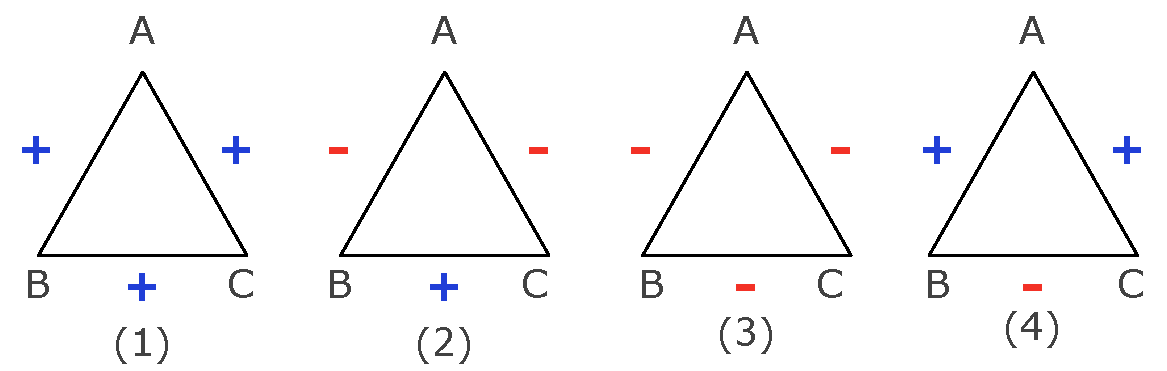
\includegraphics[height=0.8in]{Figs/strongBalance_ver.pdf}
\vspace*{-0.1in}
\caption{\label{fig:balance_strong}Classic structural balance with four different types of triads}
\end{figure}

Structural balance theory (SBT) is based on the assumption that
certain types of relationships when viewed from a local perspective
are more natural for psychological reasons~\cite{kleinberg-book}. The
local level is defined as a triangle or triad consisting of
relationships between three people.  It is natural for three people to
be friends: Alice (A) is friends with Bob (B), Bob is friends with
Chris (C) and Chris is friends with Alice. This triangle (marked (1)
in Figure~\ref{fig:balance_strong}) is considered completely
positive. Similarly, a relation where two friends, Bob and Chris have
a common enemy Alice, is also natural (triangle (2) in
Figure~\ref{fig:balance_strong}). It is considered that in such
natural relationships, there is no tension in the
interactions. However, it is less natural for Alice and Bob, and Alice
and Chris to be friends, but Bob and Chris to be enemies (triangle (4)
in Figure~\ref{fig:balance_strong}). This situation is likely to
generate tension as now Alice must avoid spending time with Bob when
Chris is around. As a result, all definitions of structural balance
would consider triangles 1 and 2 as balanced, and 4 as imbalanced.

The last type of relationship is one containing all negative
edges. This type of relationship can be considered balanced as there
is no specific conflict when three people all dislike each other but
spend no time together. As a result, in Davis's weak structural balance theory
(WSBT), triangle (3) is considered balanced~\cite{kleinberg-book}\cite{Davis:67}.  However, there is an
opportunity for one of the pairs in this triangle to become friends,
and team up against the common enemy. For this reason, (strong) SBT,
considers triangle (3) unbalanced as well~\cite{Cartwright:56}\cite{kleinberg-book}.

A complete network in which all pairs of people are connected to each
other satisfies the WSBT if all triangles in it are balanced with
respect to WSBT. In this case, the network can be divided into a set
of communities $C_1,\ldots, C_k$ such that within each community,
nodes are positively connected, and across different communities, all
connections are negative. This main result underlies many trust
inference algorithms. Algorithms that attempt to solve the {\it edge
  sign prediction problem} which involves assessing which links in a
network are positive and which links are negative, are often based on
SBT/WSBT either implicitly or explicitly.

%%  develop methods to assess
%% which nodes are likely to be connected by positive
%% edges~\cite{DuBois:2009} and which sets of nodes are
%% likely to be connected by negative edges~\cite{Leskovec:2010}. 

Guha et. al.~\cite{Guha:04} introduce one of the earliest methods that
addresses the propagation of both trust and distrust. They propose the
concepts of direct propagation, co-citation and backwards propagation,
and compute trust propagation by repeating matrix operations that
combine the three types of propagations. They report an overall $85\%$
prediction accuracy over data samples from Epinion that has equal
number of positive and negative edges.  Leskovec, Huttenlocher and
Kleinberg~\cite{Leskovec:2010} conduct a series of experiments on
three large datasets: Epinions, Slashdot and Wikipedia. In particular,
they collect two classes of features, one of which is based on degree
and the other is based on triads. These relatively local features form
a high dimensional space on which they perform standard machine
learning methods and perform edge sign predictions. Similar to our
work, they interpret some of their results in terms of the classical
balance theory~\cite{Cartwright:56}, but unlike our work, they do not
use balance theory as a starting point.

The recent work by DuBois et. al.~\cite{golbeck:distrust2011} is also
related to our paper from an algorithmic point of view. This work
stands out as it provides very good prediction performance for the
edge sign prediction problem; $80-90 \%$ on all of the three datasets
used in~\cite{Leskovec:2010} for both positive and negative edges. In this work, two
features are computed for each signed edge: the first one is based on path
probability (PP, $O(n^2)$)~\cite{DuBois:2009} and the second one uses
a force directed algorithm (FD, $O(kn)$ at each iteration where $k$ is
the average degree of the network)~\cite{golbeck:distrust2011}. In
the method of FD, the authors map trust and distrust relationships to metric
distances: the larger the distance is, the more negative (less
positive) the relation is. Then, the edge sign prediction problem is
mapped to a graph drawing problem. In this paper, we show that some of the assumptions underlying this
algorithm can be formally defined as part of a general structural
balance theory that not only works for simple positive and negative
edges, but also takes into account trust strength when
applicable. Being able to deal with strength also enables us to state
the explicit optimization criteria in the metric space for the graph
drawing problem. As a result, we are able to compare the prediction
performance with respect to an optimal placement of nodes according to
our theory. We show our method matches and outperforms the results of
this method for different data sets.

Notice that both the force directed algorithm (FD)
from~\cite{golbeck:distrust2011} and the stress majorization (SM) that
we use in this paper have been used in the field of graph
drawing~\cite{Gansner:05}. In FD, an attractive force is assigned
between endpoints of each positive edge and a repelling force is
assigned between endpoints of each negative edge. Nodes are initially
randomly laid out, and the system is simulated until a stable
equilibrium is reached when the total kinetic energy is below certain
threshold. The relation between every pair of nodes is represented by
the distance between the two end nodes in the stable layout of the
network.

While FD is simple to implement, it operates on a local pairwise
level, instead of a global level. This can lead to problems if the
local forces end up not being sufficient to hold small groups
together. Alternatively, if negative forces are too high, then the
network may continuously expand in space and the algorithm may never
converge. As a result, FD requires carefully tuned
parameters for a specific network.  In contrast, SM is a
mature approach that guarantees monotonic convergence for drawing
graphs. Moreover, in~\cite{golbeck:distrust2011}, there is no force
between pairs of unconnected nodes which can result in unintuitive
distances for such pairs. In fact as we show in our results, the FD
method maps unconnected nodes to a predominantly positive range. This
presents a problem for using this algorithm for solving the
{\it link prediction problem}~\cite{Kleinberg:03}. Link prediction is
a harder problem since networks are often sparse and one needs to find
the few edges that are true positive with high
probability. We show that our results are very promising on this
front.

In addition, to the best of our knowledge, none the existing methods
provide a principled way to study the principles underlying trust and
distrust relationships in very large networks with varying degrees of
relationship strengths. It is unclear to which degree SBT or WSBT
balance theory is valid for many large networks in which some or most
relationships are simple acquaintances~\cite{Granovetter:1973} instead
close friendship relationships. An acquaintance may not result in the
same type of structural constraints. For example, if Alice knows Bob,
and Bob knows Chris, but Chris dislikes Alice, this may not cause
much stress in the existing relationships if Alice, Bob and Chris
rarely spend time with each other, i.e. their relationship is not
strong. However, there are still some implications for the network
overall when we consider acquaintances as well as friendships. We
examine those in the next sections and provide a flexible theory of
balance that generalizes WSBT. We show that our theory allows us to
formulate convergence as an optimization problem, which can be solved
by stress majorization and illustrate that our algorithm achieves
better performance than those cited in the
literature~\cite{golbeck:distrust2011} while also providing a
principled way to approach the link prediction problem when signed
edges are present.

%%  Finally, when links are not present between
%% nodes in a network, there are multiple interpretations. It could be
%% that some nodes do not know each other or we do not know the actual
%% relationship in these cases. In both cases, we can use an inference
%% algorithm to find such edges. However, an alternate explanation could
%% be that the trust relationship is neutral, it has not yet reached a
%% point that it would be considered positive or negative. The
%% distinction in this case is that a neutral relation can become
%% positive or negative, knowing this 



\section{Extended Structural Balance Theory (ESBT)} \label{sec:esbt}
In this section, we introduce a new and more fine-tuned way to define
structural balance that we will call extended structural balance
theory, or ESBT for short. The psychological explanation for weak
structural balance relies on the concept of stress. Certain situations
cause stress in interactions and as a result, are not considered
natural. So, in balanced situations such stress must not exist. We
define this stress more precisely as a function of the strength of
relationships.

In classical balance theory, relations are restricted to binary values
($+$/$-$), which we interpret as trust and distrust. When Cartwright
and Harrary first formalized the theory of structural balance, they
also suggested that relationships of interest exist in varying
degrees, and that their theory is built on the incomplete
representation of strengths of relations~\cite{Cartwright:56}. Tie
strength is a well-studied concept in social psychology. A person may
have close friends and acquaintances (strong/weak ties), with
different trust expectations. A strong tie may represent a trust
relation corresponding constructs relevant to high risk situations,
while a weak tie may be trusted for low risk situations like providing
private information~\cite{Granovetter:1973}.

To model this distinction, we consider a scenario where relationships
have varying strengths. A strong positive link represents a close
friendship or family tie, i.e. strong trust constructs, and a strong
negative link represents hatred, i.e. strong distrust
constructs. However, many other types of trust relationships may exist
in between the spectrum of (strong) trust and (strong) distrust. For
example, a negative bias may be considered a weak distrust and a weak
tie may represent weak (positive) trust.
 
A complete balance theory should be able to deal with relationhips
with strengths.  As a first step, we need to have a measurement of
relations with various strengths. While it is arguable whether
such strengths can be expressed by numerical values, it is fairly
clear that the strength of any two relations can be compared. For
positive relations such as liking, valuing or approving, two
relationships are comparable in terms of which one is stronger than
the other. Similar argument applies to two negative
relations. Finally, a positive relation and a negative relation are
comparable by their signs. Hence, relations with strengths by nature
inherit a total ordering.
 
Let the collection of relations with strengths be $E$. An edge $(A,B)$
and a relation with associated strength $e$ will be used
interchangeably in later discussion. We pick the ordering $\preceq$
such that, $e_{1} \preceq e_{2}$ denotes $e_{1}$ is positively
equivalent to or stronger than (or negatively equivalent to or weaker
than resp.) $e_{2}$. That is, if $e_{1}, e_{2}$ are both positive
relations, $e_{1} \preceq e_{2}$ if $e_{1}$ is at least as positive as
$e_{2}$ in terms of strengths; if $e_{1}, e_{2}$ are both negative
relations, $e_{1} \preceq e_{2}$ if $e_{1}$ is at most as negative as
$e_{2}$ in terms of strengths; if $e_{1}, e_{2}$ are of different
signs, $e_{1} \preceq e_{2}$ if $e_{1}$ is positive and $e_{2}$ is
negative. In the simplest case where we have only positive and
negative relations, we have that $+ \preceq -$. 
 
We also consider a {\bf neutral relationship} as one that is unbiased,
which will be denoted as $O$. Basically a neutral relationship is a
non-negative and non-positive relationship, corresponding to no
opinion and no bias. In the case of incomplete networks,  classic balance theory implicitly considered two types of triads with
neutral relations balanced: ``$+, +, O$",
``$+,-,O$"~\cite{kleinberg-book}. With the introduction of neutral
relations, $E$ can be partitioned into three subsets: positive
relationships $P$, negative relations $N$ and neutral relations
$O$. Following the definition of ordering $\preceq$, it is clear that
for any $e_{+} \in P$, $e_{O} \in O$, $e_{-} \in N$, $e_{+} \preceq
e_{O} \preceq e_{-}$ holds. We use $\tuple{e_1}{e_2}$ to denote the
set of relations $\tuple{e_1}{e_2}$ = $\{e\:\mid\: e_1\preceq e\preceq
e2\}$. Hence, given $\tuple{e_1}{e_2}$, the lower bound $e_1$
represents the strongest possible relationship and the upper bound
represents $e_2$ represents the weakest possible relationship in this
range.
 
\subsection{Principles of Structural Balance}
A triad is the smallest unit in balance theory, within which two of
its relations cause influence over the third one.  Such an influence
will limit the range of comfortable relations of the third relation in
a balanced state; and if it goes out of range, tension occurs and
participants will suffer from {\bf stress}. Participants will seek
relationship changes to resolve this type of stress. We call such range
of relations {\bf tolerance}, with which we interpret structural
balance at a finer level.

Given a network of nodes $G=(V,E)$, there exists a tolerance for each
pair $(A,B)$ of nodes of the form $\tuple{e_1}{e_2}$ which is
constrained by the triads $(A,B)$ is part of. When there is no
constraint, i.e. stress, on a specific relationship, the tolerance
includes any relationship in $E$. We propose two principles regarding
tolerance: transitivity and heterophily.

\begin{principle}[Transitivity of positive relationships]
Let individuals $A$, $B$, $C$ in a network form a traid, and $(A,B)$,
$(A,B)^{'}$, $(B,C)$ be positive. Suppose $T=\tuple{e_1}{e_2}$ denotes
the tolerance of $(A,C)$ based on relations $(A,B),(B,C)$, and
$T'=\tuple{e_1'}{e_2'}$ denotes the tolerance based on
$(A,B)^{'},(B,C)$. If $(A,B)' \preceq (A,B)$ then we have that
$e_2'\preceq e_2$.

Furthermore, there exists a $e_{sp} \in P$ such that if $(A,B)\preceq
e_{sp}$ and $(B,C) \preceq e_{sp}$, then $e_{2} \preceq e_{O}$ holds
for all $e_{O} \in O$. That is, $T$ will only have positive relations
beyond a certain threshold $e_{sp}$.
\end{principle}
In other words, the fact that B are friends with both A and C provides
the freedom for $A$ and $C$ to become friends; and there is stress on
$A$ and $C$ to get close. The stronger the relation between $(A,B)$
and $(B,C)$, the higher the stress between $(A,C)$ to be connected
(more) positively, and the resulting tolerance is restricted to be
more positive.

The stress that is based on positive relations has been frequently
defined by SBT and WSBT. Positive relations in a triad cause stress
for the remaining relations to be positive. As a result, both in SBT
and WSBT, a balanced network consists of communities that are
connected to each other with positive ties. When we consider the
strength of relations, we generalize this by saying that the more
positive two of the relations are in a tie, there is lesser tolerance
for negative trust values.

There is a point when the strength of the two positive relations are
strong enough such that it is imbalanced for $(A,C)$ to remain
unfriended, i.e. neutral. This observation is inspired by the ``strong
triadic closure" in~\cite{kleinberg-book}. In trust literature, it is
often referred as the ``transitivity of trust'' though transitivity is
also used in other contexts.

\begin{principle} [Heterophily in relationships] 
Let individuals $A$, $B$, $C$ in a network form a triad. Suppose
$T=\tuple{e_1}{e_2}$ denotes the tolerance of $(A,C)$ based on
relations $(A,B),(B,C)$, and $T'=\tuple{e_1'}{e_2'}$ denotes the
tolerance based on $(A,B)^{'},(B,C)$. We have that if
$(A,B)' \preceq (A,B) \preceq (B,C)$, or $ (B,C) \preceq (A,B) \preceq
(A,B)'$, then $e_1\preceq e_1'$.

Furthermore, suppose there is a well-defined concept of difference
between two relations with strengths. Then, the larger difference
between $(A,B)$ and $(B,C)$ is, less positive $e_1$ (the lower bound)
is.
\end{principle}
Given individuals $A$, $B$, $C$ in a network, if the relationship
between $(A,B)$ and the relation between $(B,C)$ differs to some
extent, then the tolerance is geared towards the
negative. Furthermore, the more different the strength of the
relationships are, the tolerance is geared towards more
negative values. 

The second type of stress is an interpretation of homophily. We note
that homophily, i.e. having common friends or enemies, may sometimes
cause stress (in $+,+,+$) but sometimes it does not (in $-,-,-$ for
WSBT). However, lack of homophily, which we call heterophily does
cause stress. For example, consider the case $+,+,-$ for $(A,B)$,
$(B,C)$ and $(A,C)$. There is stress on $(A,C)$ to be positive due to
transitivity. But, there is also stress on $(A,B)$ and $(B,C)$ to be
negative. Either way, the result will be more desirable: either all
being friends, or having two friends with a common enemy. We call the
second type of stress the principle of heterophily. The more different
the ties are (the strongest difference is between distrust and trust,
and the weakest difference is between two identical trust ties), the
more pressure there is for the tie to be negative.  At a point when
the difference between $(A,B)$ and $(B,C)$ is significant enough, we
argue that a positive value for $(A,C)$ will cause imbalance. This is
inspired by the observation that two people who have severely
conflicted relationships with a common neighbor, e.g., one is the
other's close friend's enemy, are not likely to be friends.

\begin{table}[h]
\begin{center}
 \begin{tabular}{cc|cl} 
  $(A,B)$ & $(A,C)$ & Tolerance for $(B,C)$ &  \\ \hline
  $+$ & $+$ & $\tuple{+}{O}$ & Transitivity \\
  $+$ & $-$ & $\tuple{O}{-}$ & Heterophily \\ 
  $-$ & $-$ & $\tuple{+}{-}$ & No stress \\ 
 \end{tabular}\\  \vspace{1mm}
\caption{\label{ref:classic_balance}Tolerance rules in structural balance theory}
\end{center}
\end{table}

The two principles help interpret balance in terms of relations with
strengths precisely. A triad is balanced if all relationship strengths
are within the tolerance implied by the other relationships in the
triad.

\begin{definition} [Balance]
A triad $A,B,C$ is balanced if for all pairs $(A,B)$, given the
tolerance $\tuple{e_1}{e_2}$ of $(A,B)$ with respect to $(B,C),(A,C)$,
we have that $(A,B)\in \tuple{e_1}{e_2}$. 
Given a network $G$ of relationships, $G$ is said to be balanced if
for all triads in the network are balanced.
\end{definition}

The tolerance rules for the Davis's balance theory are
given in Table~\ref{ref:classic_balance}. Notice that neutral
relations ``$O$" are also added. This is because triangles ``$+, +,
O$" and ``$+, -, O$" are allowed implicitly in their theory in the
general case of incomplete graphs. According to the table, triads (1), (2) and
(3) from Figure~\ref{fig:balance_strong} are balanced as each relation
strength is within the tolerance, but triad (4) is not
balanced. Hence, our theory generalizes WSBT in the
classical balance theory.

\subsection{Balance theorems with weak and strong ties.} \label{sec:weak_strong}
In this section, we show how our reasoning can be applied to a network
with multiple types of relationships. We consider a set of discrete
labels (shown in Table~\ref{ref:rel_types}) that have been discussed
in previous literature and show that we can reason about balance in
such a network using our two principles. 

{\bf Strong positive ties, s+ (trust)} are similar to a close
friendship. There is a strong expectation of reciprocity, similarity
of tastes (homophily), common intentions and benevolence towards each
other~\cite{Tomasello:2005}. The traditional definition of SBT is
based on these types of positive relationships.

{\bf Strong negative ties, s- (distrust)} are generally explained as
having negative experiences with someone which is indicative of their
negative intentions, unreliability and overall belonging to groups
that are not considered trustworthy~\cite{Fiske:2007}. Even when a
distrusted person behaves in a trustworthy way, this could be
considered a trick to get one to trust them.

\begin{table} [htbp!]
\begin{center}
\begin{tabular}{p{1.6in}p{1.6in} }
Relation Type & Interpretation \\ \hline
Strongly positive (s+) & close friendship, trust  \\ 
Weakly positive (w+) & aquiantance \\
Neutral (O) & unbiased relation, no relation  \\
Weakly negative (w-) & minor disagreement, negative bias  \\
Strongly negative (s-) & hatred, distrust  
\end{tabular}\\\vspace{1mm}
\caption{\label{ref:rel_types}Strength of relations: $s+\preceq w+\preceq O\preceq w- \preceq s-$.}
\end{center}
\end{table}

However, these are not all the different classes of relationships that
one might consider in a network. While one might consider a continuum
of tie strength, we summarize some additional discrete classes. {\bf
  Weak positive ties, w+ (weak trust)} can be considered a utilitarian
type of trust. Interacting with someone who is only trusted partially is
more risky, but can be acceptable in certain situations. For example,
Uzzi~\cite{Uzzi:1996} uses the term embedded vs. arm's length ties to
distinguish between the two types of trust. While a close friend is
highly trusted, they may not have access to the resources a more risky
contact may provide. Granovetter~\cite{Granovetter:1973} uses the term
weak tie to talk about a relationship that is an acquaintance, not a
close friend. Weak ties give access to less privileged information
than strong ties, but come from outside of one's close network. In
both cases, there is a trust relationship between two people, but this
does not imply a continuous interaction or a strong affective
component as in trust.

We also introduce {\bf weak negative ties, w- (weak distrust)} to
model cases in which there is a certain amount of distrust as a result
of biases stemming from social groups people belong to or heresay that
may not be as strong as distrust~\cite{Ames:2011}. In essence, the
burden of proof of one's trustworthiness is much higher in distrust
than in weak distrust, but in both cases, positive evidence is not
evaluated in the same way as in trusting relations. These five types
of relationships are summarized in Table~\ref{ref:rel_types}.


\begin{table}[htbp!]
\begin{tabular}{p{1.6in}|p{1.2in}}
 \begin{tabular}{p{0.3in}p{0.3in}p{0.5in}} 
$(A,B)$ & $(A,C)$ & $(B,C)$'s tolerance \\ \hline
$s+$ & $s+$ & $\tuple{s+}{w+}$ \\
$s+$ & $w+$ & $\tuple{s+}{O}$  \\
$s+$ & O & $\tuple{s+}{w-}$ \\
$s+$ & $w-$ & $\tuple{O}{s-}$ \\ 
$s+$ & $s-$ &   $\tuple{w-}{s-}$ \\
$w+$ & $w+$ & $\tuple{s+}{w-}$ \\
$w+$ & O & $\tuple{s+}{s-}$ \\
& & 
\end{tabular} &
\begin{tabular}{p{0.3in}p{0.3in}p{0.5in}} 
$(A,B)$ & $(A,C)$ & $(B,C)$'s tolerance \\ \hline
$w+$ & $w-$ & $\tuple{w+}{s-}$ \\
$w+$ & $s-$ & $\tuple{O}{s-}$ \\ 
O & O & $\tuple{s+}{s-}$ \\ 
O & $w-$ & $\tuple{s+}{s-}$ \\ 
O & $s-$ &  $\tuple{w+}{s-}$ \\ 
$w-$ & $w-$ & $\tuple{s+}{s-}$ \\ 
$w-$ & $s-$ & $\tuple{s+}{s-}$ \\ 
$s-$ & $s-$ & $\tuple{s+}{s-}$ \\
\end{tabular}
\end{tabular} \\\vspace{1mm} 
\caption{\label{tab:weak_strong_tolerance}Tolerance of strong, weak \& neutral relations}
\end{table}

Given these relationship types, we now describe the tolerance for
different triads in Table~\ref{tab:weak_strong_tolerance} and the
resulting imbalanced triads or structures in
Table~\ref{tab:imbalanced_extended}. Notice that the triads with
two positive relations and one negative relation are imbalanced as
they are in classic balance theory, except for the cases in which all
three relations as weak. In fact, the types of triads that consist
of weak relations and neutral relations only are not considered to be
imbalanced structures. The argument here is that when all relations
are weak or neutral, the influence inside the triad is not significant
enough to draw tension. Also, triads of type ``$s+$ $s+$ O" and
``$s+$ $s-$ O" are considered to be imbalanced structures. The
arguments against each type of imbalanced structure is listed in
Table~\ref{tab:imbalanced_extended}.

\begin{table}[htbp!]
\begin{center}
 \begin{tabular}{p{3in}}
Triads and  the argument for stress \\ \hline
$(s+ s+ s-)$ $(s+ s+ w-)$ $(s+ w+ s-)$ $(s+ w+ s-)$ $(w+ w+ s-):$ \\
my two friends cannot get along with each other \\ \\

$(s+ s+ O)$: my two close friends do not friend each other \\ 
$(s+ s- O)$: my enemy's close friend does not pick a side\\ 
\end{tabular} \vspace{4mm}
\caption{\label{tab:imbalanced_extended}Imbalanced triadic structures
  in the presence of strong and weak ties.} 
\end{center}
\end{table}
\vspace*{0in}

\subsection{Relation Distance and General Expression of Balance}
The concept of extended balance is meaningful only if the tolerance
rules can be explicitly defined, so that whether a triad and a network
is balanced or not can be determined. Whenever relations
are drawn from a finite and small set, this is easy to do. However, it
is considerably more complex in the general case when the strengths
of relations are drawn from arbitrary numerical values. 

To handle such cases, we refine the measurement of relations with
strengths from a total ordering to positive real values. In
particular, we define function $\psi: E \rightarrow R^{+}$ such that,
for two relations $e_{1}, e_{2} \in E$, $\psi(e_{1}) \leq \psi(e_{2})$
if and only if $e_{1} \preceq e_{2}$.  Since positive values can be
seen as metric distances, we call $\psi(e)$ the relation distance of
$e$.  In other words, relations with varying strengths are represented
by distances with different lengths.  More negative strengths are
represented by larger distances and more positive strengths are
represented by smaller distances. We propose the following general
rule of tolerance with the concept of relation distance.


%% In the case of WSBT, Table 1 set up
%% such tolerance rules. In the extended case when strong/weak ties are
%% introduced, Table 3 provides the tolerance rules. For general cases
%% when relation strengths are not limited to particular types, however,
%% the tolerance rules are not defined. We address this problem by
%% expressing relation in terms of metric distance, based on which we set
%% up a uniform tolerance rule that generalizes Table 1 and 3.

%% In previous discussion, relations are measured by a complete
%% ordering. To express it as distance, we need an additional assumption
%% that the difference between any two relation strengths are well
%% defined. We introduce a function from relation to real values: $\psi:
%% E \rightarrow R^{+}$. For each relation $e \in E$, $\psi(e)$ denotes
%% its distance expression, which will be called relation distance for
%% simplicity. The ordering relation is then reduced to the numerical
%% comparing operator $<$.  In particular, $\psi(e_{1}) < \psi(e_{2})$ if
%% and only if $e_{1} \preceq e_{2}$.


\begin{definition} \label{def:gen_tolerance}
Given adjacent relations $(A,B)$ and $(B,C)$, the tolerance of $(A,C)$
is given by $[|\psi(A,B)-\psi(B,C)|, \psi(A,B)+\psi(B,C)]$.
\end{definition}

It can be easily checked that the general tolerance rule agrees with
Principle 1 and 2 by substituting $\leq$ for $\preceq$.  Immediately, we have the following
theorem.
\begin{theorem} 
Given a triad $(A,B,C)$, if $\psi(A,B)$, $\psi(B,C)$, $\psi(A,C)$
satisfies the metric triangle inequality, then $(A,B,C)$ is balanced.
\end{theorem}

To illustrate how the distances can be used to represent a given set
of strength values, we revisit WSBT. Consider two thresholds:
$b_{+} < b_{-}$ such that if $\psi(e)\geq b_{-}$ then the relationship
$e$ is negative. Similarly, if $\psi(e)\leq b_{+}$, then $e$ is
a positive relationship. For any value $b_{+} < \psi(e) < b_{-}$, the
relationship is considered neutral. We can see that as long as
$b_{-}>2b_{+}$, Table~\ref{ref:classic_balance} is equivalent to
Definition~\ref{def:gen_tolerance}.

\begin{figure}[th]
\centering
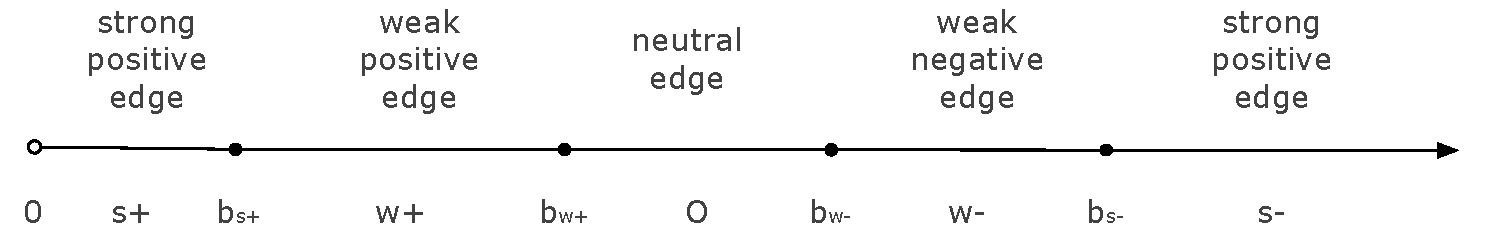
\includegraphics[height=0.55in]{Figs/mapping2.pdf}
\vspace*{-0.1in}
\caption{\label{fig:partition}Partitioning of distances:
  $(0,b_{s+}]:s+$, $(b_{s+}, b_{w+}): w-$, $[b_{w+}, b_{w-}]:O$,
$(b_{w-}, b_{s-}):w-$, and $ [b_{s-}, \infty):w+$.}

\end{figure}

Similarly, to capture the example from Section~\ref{sec:weak_strong},
we consider the partitioning of the distance domain given in
Figure~\ref{fig:partition}. We can see that if the following
conditions are satisfied for the boundary parameters: 

\begin{tabular}{p{1.5in}p{1in}}
$b_{w+}  > 2b_{s+}$ & $b_{s-}  > b_{w-} + b_{s+}$  \\
$b_{s-}  > 2b_{w+}$ & $b_{w-}  > b_{w+}+b_{s+}$
\end{tabular} 

\noindent the tolerance given in
Table~\ref{tab:weak_strong_tolerance} are equivalent to
Definition~\ref{def:gen_tolerance}, and all triads shown in
Table~\ref{tab:imbalanced_extended} are imbalanced according to metric triangle
inequality.




\section{Convergence Model} \label{sec:mathmodel}
Researchers have long argued that every social network has a tendency
towards balanced states~\cite{Doreian:02}.  The next question of
interest is if an imbalance rises, in what way will a social network
change towards a new balance.  It is noted in social psychology
literature that people are reluctant to make changes in relations as
they tend to avoid the effort needed to make such changes. In a balanced
triadic relation, participants are likely to do nothing and keep their
pairwise relations as what they were. In an imbalanced triadic
relation, participants are likely to make the smallest effort possible
to regain triadic balance. We define the concept of relation cost as
the effort one needs to take to accomplish a certain relation
change. Our convergence model is established based on a unified
assumption: every social network converges in a way that requires as
little total change in relations as possible to reach a balanced
state.

With the concept of relation distance, we are able to express the
structure of a social network by drawing it in the Euclidean
space. The strength of each relation is expressed by the distance
between their locations. Notice that every layout in the Euclidean
space automatically satisfies the metric triangle inequality, and
hence corresponds to a balanced state of the network.  For an
imbalanced social network, it is not possible to draw it using its
initial relation distances.  Hence, our convergence model produces a
layout of the social network with minimum total relation cost from the
original one.

Let $G=(V,E)$ denote an arbitrary social network, and $G^{*}=(V,
E^{*})$ denote a balanced state of $G$. Let $n*n$ matrix $X$ denote
the layout of $G^{*}$, with each row vector $x_{i}$ denoting node
$i$'s location in $m$-dimensional space. For each pair $(i,j)$,
$\psi(i,j)$ denotes its relation distance in $G$, and $d_{i,j}(X)$
denotes distance between $i$ and $j$ in $X$, i.e., its relation
distance in $G^{*}$.  Given an edge $(i,j)\in E$, the
relation cost on $(i,j)$ is given by:
\[c_{i, j}(X)=w_{\psi(i,j)}*(d_{i,j}(X)-\psi{(i,j)})^2\]
where the weight value is a function of the original distance. The
weight function can take into account the difficulty of changing a
relation. For example, it is generally easier to change a neutral
relation than a positive or a negative relation that incorporate an
initial bias. The study of optimal weights is beyond the scope of this
paper. However, we consider three main classes of weights:
\[
 w_{\psi(i,j)}= \left\{ 
  \begin{array}{l l}
    w_{+} & \quad \text{if $\psi(i,j)$ is a positive edge}\\
    w_{O} & \quad \text{if $\psi(i,j)$ is a neutral edge}\\
    w_{-} & \quad \text{if $\psi(i,j)$ is a negative edge}\\
  \end{array} \right.
\]

If $w_{O} << w_{+}$ and $w_{O} << w_{-}$, then neutral edges would
have very little influence on the already established
positive/negative relations.

\begin{definition}
Let $G=(V,E)$ be a social network where $E$ is a set of weighted
edges. Its converged network $G^{*}=(V,E^{*})$ is given by layout
matrix $X$ with $d_{i,j}(X)$ as the relation distance between every
pair $(i,j)$, such that the total relation cost $\sigma(X)$ is
minimized:
\[\sigma(X)= \min_{X} \sum_{i<j \leq n}w_{\psi(i,j)}*(d_{i,j}(X)-\psi{(i,j)})^2\]
\end{definition}

The optimization of relation cost is in fact a Metric
Multidimensional Scaling problem (MDS) by assigning nodes a location
in metric space. The total cost function is called stress in MDS, and
is often minimized through an optimization strategy called {\it stress
  majorization} \cite {Gansner:05}. Stress majorization is an iterative
method that guarantees monotonically decreasing stress in each
iteration, and returns a locally minimum solution.  It is recognized
as a principled technique in the field of graph drawing. The
algorithm, however, requires $O(n^3)$ time and $O(n^{2})$ space. Due
to its complexity, stress majorization is applicable on graphs with
limited size. We are in the process of developing an approximation
method for this problem as a result. In this paper, however, we will
investigate the performance of the exact solution to stress
majorization.





\begin{figure*}[thbp!]
\centering
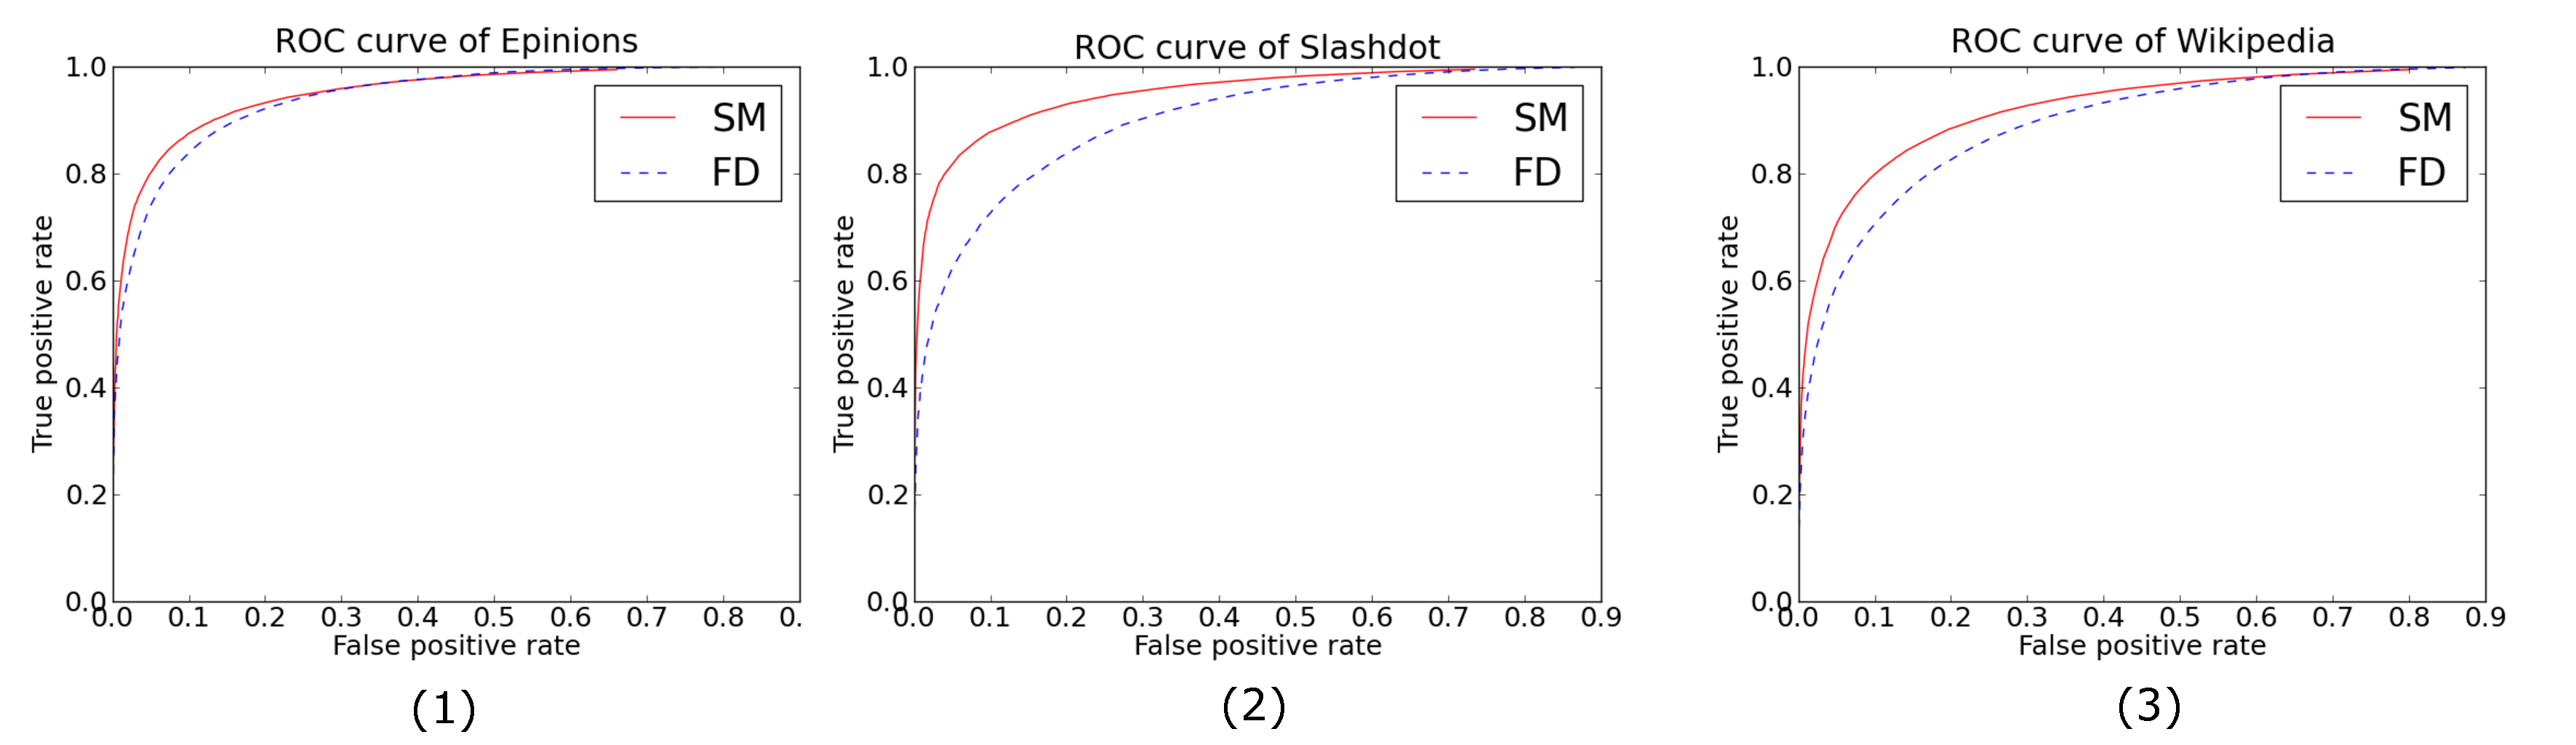
\includegraphics[height=2in]{Figs/ROC_curve_hor.pdf}
\vspace*{-0.1in}
\caption{\label{fig:ROC}The ROC curves are drawn upon distances of
  hidden edges, generated by SM and FD for (1) Epinions, (2) Slashdot
  and (3) Wikipedia datasets.}
\end{figure*}


\section{Experimental Results} \label{sec:results}
In this section, we first focus on the {\it edge sign prediction
  problem}. Suppose we are given a social network with signs, but a
small fraction of the edge signs are ``hidden''. How can we predict
these signs with the information provided by the rest of network?
The convergence model is able to predict these ``hidden'' signs. Let's
denote the original social network with all signed edges as $G$, the
network consisting of hidden edges as $G_{h}$, and the network
consisting of the remaining edges as $G_{r}$. The edges (relations)
between each pair of nodes is measured by $\{+,\,-,\,O\}$. We run the
convergence model on $G_{r}$, and denote the network after convergence
as $G_{r}^{'}$. We expect that the signs of the hidden edges in
$G_{r}^{'}$ largely agree with the true signs.

By the assumption that every social network has a tendency towards
balance, it can be inferred that $G$ is largely balanced at any
moment. Hence, the majority of $G_{r}$ is balanced. The only
exceptions are the components with hidden edges, which are of sign $O$
in $G_{r}$. By the principle of total relation cost minimization, the
changes mostly occur on the $O$-sign hidden edges during the
convergence. We expect the hidden edges in $G_h$ to have their
true signs in $G_{r}^{'}$ if $G$ is largely balanced.

We compare our algorithm to force directed algorithm (FD)
in~\cite{golbeck:distrust2011}. Note that we have tuned our
implementation of FD to provide similar performance reported in this
work. Even though this work combines two algorithms, in our comparison
experiments, we find that FD alone gives equally good prediction
performance on all three datasets as the combination. Due to space
limitations, we exclude the detailed study of PP and FD/PP combination
from this paper.


\begin{algorithm}\label{alg}
 \KwData{$M, k, deg, G$}
 \KwResult{$Pt, Nt$}
 Get $G'=$ generate-subgraph$(M, k, deg, G)$\;
 Partition $G'$ into 10 groups of test and training samples\;
 Create two empty sets $Pt$, $Nt$\;
 \For{each of the groups}{
 run SM on the training sample and get the layout\;
 \For{each edge e in the testing sample}{
 compute its distance in the layout\;
 \eIf{e is a positive edge}{
   add its distance to $Pt$\;
   }{
   add its distance to $Nt$\;
  }
 }
 }
 \caption{SM Prediction}
\end{algorithm}

We use the same three datasets as it is
in~\cite{golbeck:distrust2011}~\cite{Leskovec:2010} to conduct our
experiments, all provided by the Stanford Large Network Dataset
Collection. (1) {\em Epinions} is a product review website where users
give reviews and ratings on product articles. Users can choose to
trust or distrust others. The network contains more than 100,000 users
and over 700,000 trust/distrust edges. (2) {\em Slashdot} is a
technology news website where users rate each other as friends or
foes. The dataset released in February 2009 contains over 77,000 users
and over 900,000 friend/foe edges. (3) {\em Wikipedia} elections
collects the votes by Wikipedia users in elections for promoting
candidates as administrators. Each user can give a supporting
(positive) or opposing (negative) vote on the promotion of
another. The dataset has about 7,000 users and around 100,000 votes
(edges).

All edges are treated as undirected. Running SM on the entire dataset
is infeasible due to both the memory and computational cost. As a
result, we generate random samples of our datasets using snowball
sampling method in which a small number $k$ of seeds with degree
greater than a given threshold $deg$ are selected at random, then all
nodes that are adjacent to the seed node are selected iteratively
until the desired network size is reached.  In our practice, the size
of the resulting graph is in the range 3,000-5,000 nodes, $k$ is
chosen from 2-10 randomly and $deg$ is chosen from 7-20 randomly. For
each dataset, we generate 10 sub-networks and perform 10-fold cross
validation. The number of edges in a sub-network of Epinions is around
180,000, for Slashdot 65,000 and for Wikipedia 160,000. In the
implementation of SM, the partitioning of the distance domain
satisfies $b_{+} < 1/2b_{-}$, conforming to our theory. The weight of
each type of edge satisfies $w_{O}<<w_{+}<1/2w_{-}$. The first
inequality has been argued in the previous section. The second one is
chosen empirically, indicating that a negative edge has larger
influence than a positive one. We use the same setting for all the
networks and do not employ any other adjustable parameters.


\begin{figure*}[thbp!]
\centering
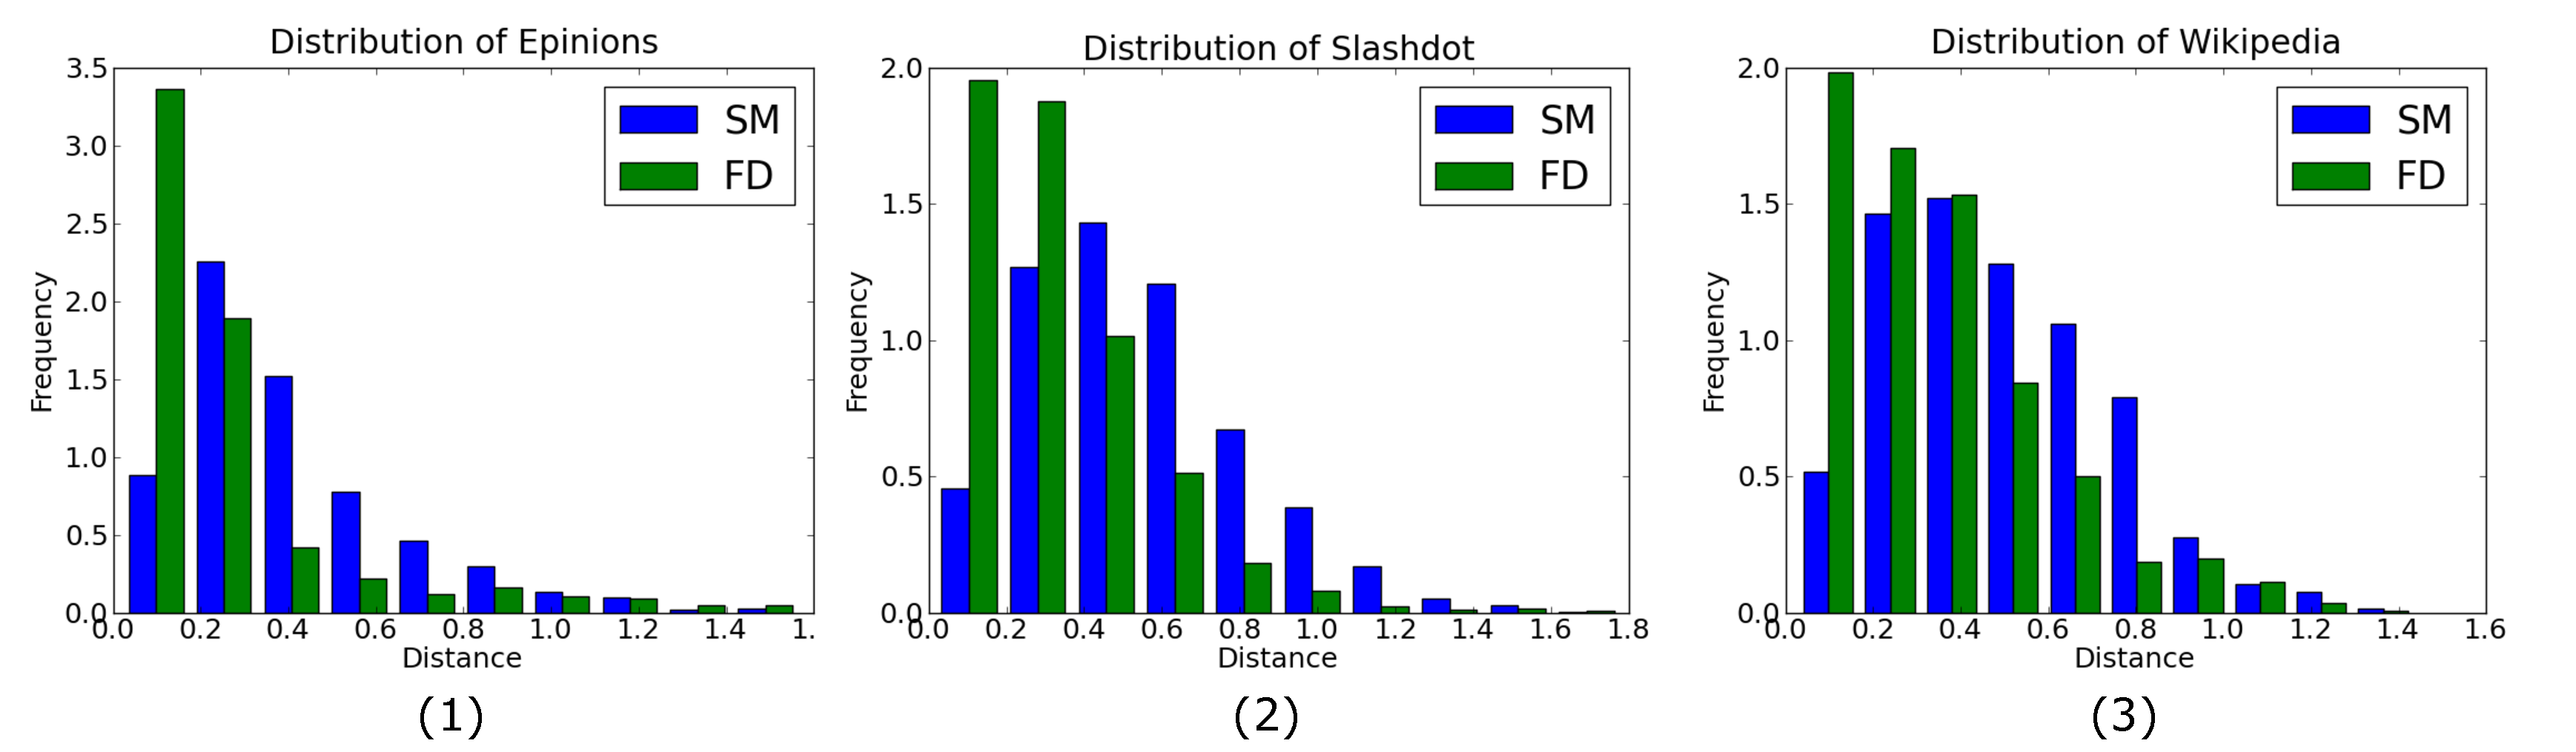
\includegraphics[height=2in]{Figs/hist1_hor.pdf}
\vspace*{-0.1in}
\caption{\label{hist}The histograms are drawn upon distances of
  neutral testing edges, generated by SM and FD for (1) Epinions, (2)
  Slashdot and (3) Wikipedia datasets.}
\end{figure*}

\noindent {\bf Edge Sign Prediction.} The distances of testing edges
are computed by the layout of the training data. Given a distance
threshold, the sign of each edge is predicted as positive if and only
if its distance is smaller than the threshold. In the previous work,
such threshold is computed from the (distance,sign) pairs of the
training samples using standard machine learning
techniques~\cite{golbeck:distrust2011}\cite{Leskovec:2010}. In this
paper, however, we do not concentrate on the learning process. The
issue of interest is how good the convergence model performs in
separating hidden positive edges from negative ones in terms of
distance. Instead of making predictions based on a particular
threshold, we draw ROC curves for evaluation which capture the
performance of sign prediction for both positive and negative edges
across all thresholds and compute the false and true positive rates
based on the computed $Pt$ ($Nt$) values returned by the
Algorithm~\ref{alg}. The ROC curves in Figure~\ref{fig:ROC} are drawn
upon the $Pt$ ($Nt$) values from the accumulation of all testing
samples.

For all three datasets, we find the ROC curve of $SM$ is on the
``northwest'' side of the one of $FD$, which indicates $SM$ is
consistently better than $FD$ in separating hidden positive edges from
negative ones. Notice that the improvement for Slashdot is the most
significant one among the three, possibly due to the fact that
Slashdot edges represent ``friends'' or ``foes'', which is by nature a
more clear identification of trust/distrust compared to votes in
Wikipedia or distrust for reviews in Epinions.  As a result, our
convergence model produces a very good prediction performance.  On the
Epinions and Slashdot datasets, the best thresholds on ROC curve give
$88-90 \%$ accuracy on both positive and negative hidden edges. For
Wikipedia, $SM$ achieves $83-85 \%$ at the best threshold. The
accuracy rates of Epinions and Wikipidea match the best results from
previous work, and Slashdot appears to be the best so far.

\noindent {\bf General Link Prediction.} The {\it edge sign
  prediction} only deals with the cases in which we already know that
an edge exists in the original network. A more general and harder
problem is to predict whether there is a positive or a negative edge
between a pair of nodes (link prediction~\cite{Kleinberg:03}). The
difficulty of these problems stem from the fact that social networks
are usually sparse with a lot more neutral relations than biased
relations. Our convergence model should be able to make general edge
predictions based on distances. If larger distances represent more
negativeness (less positiveness), then the distance of a neutral
relation should be smaller than a negative one and larger than a
positive one. As a consequence, the distribution of neutral edges in
terms of distance should concentrate in the middle range. We study
this distribution, as a preliminary step towards solving the general
edge prediction.

For each dataset, we generate samples based on random source nodes as
before, except that we exclude the edges between the $k$ source
nodes. Instead of cross validation, we use the entire sub-network for
training, and use the $k(k-1)/2$ edges between the $k$ source nodes as
testing data, whose signs are available in the original dataset
(positive, negative or neutral, i.e. no link). %% Similarly, the signs of
%% the testing edges should not be influenced strongly by the other edges
%% in the network. Hence, a
After convergence the distances of these edges should be
representative of their true signs. We repeat the experiments 50 times
over all three datasets, and collect the distances for only the
neutral testing edges. Figure~\ref{hist} shows that the distances of
neutral testing edges generated by SM do relatively concentrate in the
middle-range of values following an almost Gaussian distribution. In
contrast, the majority of neutral testing edges's distances by FD have
small values, implying a positive prediction is much more likely for
FD than for SM.  However, SM provides more flexibility as the
distances are distributed over a larger range with an almost Gaussian
distribution, allowing us to test different tunable algorithms.
%% The experimental results show the superiority of our convergence model
%% in predicting signed edges. Moreover, they justify that our general
%% balance theory is a relatively accurate description of the stable
%% state of social networks, and that the convergence model correctly
%% characterizes the dynamics of social network.
As a result, our model
is a good starting point for developing algorithms for solving the general
{\it link prediction problem}.


\section{Conclusions} \label{sec:conclusions}
In this paper, we introduced a general model for structural balance
theory that can handle relation strengths and generalizes the
classical balance theory. We showed that our notion of balance can be
mapped to triangular inequality over metric distances and the issue of
convergence can be modeled as the metric multidimensional scaling
problem for which stress majorization provides exact solutions. We
have shown that our theory can be used to effectively solve the edge
sign prediction problem and its performance matches and exceeds state
of the art for this problem. This is due to the fact that positive and
negative edges are mapped to a continuous range of strengths based on
the constraints provided by the other nodes. However, in contrast with
previous work, our method is aware of global constraints based on
balance which results in better results overall. Furthermore, the
solutions provided by our method can also be used to solve the harder
{\it link prediction problem}.

We are investigating various avenues of future work. An approximation algorithm
of stress majorization has been developed in the context of social networks.
Furthermore, we are currently testing how the inclusion of relation
strength improves performance by considering other actions of the
users that imply the existence of a social tie. Our method also has
applications to many related problems like clustering and link
prediction, which we are currently investigating. We are studying the
various properties of our theory in general networks and how it can be
extended to an asymmetric interpretation of links.  Our method also
allows us to study and compare the characteristics existing networks
towards balance such as the ratio between positive and negative
distances, distribution of neutral edges. These measures can help us
develop new insights into the nature of adversarial relationships in
different networks.

%% \section*{Acknowledgments}
%% Research was sponsored by the Army Research Laboratory and was
%% accomplished under Cooperative Agreement Number W911NF-09-2-0053. The
%% views and conclusions contained in this document are those of the
%% authors and should not be interpreted as representing the official
%% policies, either expressed or implied, of the Army Research Laboratory
%% or the U.S. Government. The U.S. Government is authorized to reproduce
%% and distribute reprints for Government purposes notwithstanding any
%% copyright notation here on.

%% We also would like to thank T. DuBois for sharing the implementation
%% details of his algorithm.






% trigger a \newpage just before the given reference
% number - used to balance the columns on the last page
% adjust value as needed - may need to be readjusted if
% the document is modified later
%\IEEEtriggeratref{8}
% The "triggered" command can be changed if desired:
%\IEEEtriggercmd{\enlargethispage{-5in}}

% references section

% can use a bibliography generated by BibTeX as a .bbl file
% BibTeX documentation can be easily obtained at:
% http://www.ctan.org/tex-archive/biblio/bibtex/contrib/doc/
% The IEEEtran BibTeX style support page is at:
% http://www.michaelshell.org/tex/ieeetran/bibtex/
%\bibliographystyle{IEEEtran}
% argument is your BibTeX string definitions and bibliography database(s)
%\bibliography{IEEEabrv,../bib/paper}
%
% <OR> manually copy in the resultant .bbl file
% set second argument of \begin to the number of references
% (used to reserve space for the reference number labels box)

\bibliographystyle{IEEEtran}
\bibliography{trust}




% that's all folks
\end{document}


